	\documentclass[12pt]{article}

%% Language and font encodings
\usepackage[english]{babel}
\usepackage[utf8x]{inputenc}
\usepackage[T1]{fontenc}

%% Sets page size and margins
\usepackage[a4paper,top=2cm,bottom=2cm,left=2cm,right=2.5cm,marginparwidth=1.75cm]{geometry}

%% Useful packages
\usepackage{amsmath}
\usepackage{amsfonts}
\usepackage{graphicx}
\usepackage[colorinlistoftodos]{todonotes}
\usepackage[colorlinks=true, allcolors=blue]{hyperref}

\title{Homework 6}
\author{Motoaki Takahashi}
\date{}

\begin{document}
\maketitle
\section*{Question 1}
Given the initial stock of lumber $k_{0}$, let $\mathcal{K}=[0, k_{0}]$ be the set of possible values for a stock of lumber, and  let $\mathcal{P}=\mathbb{R}$ be the set of possible prices. $\mathcal{K}\times\mathcal{P}$ is the state space. Let $(k, p)\in\mathcal{K}\times\mathcal{P}$. Then the Bellman equation is
\begin{equation}
    V(k, p)=\max_{k'} p\cdot (k-k')-0.2(k-k')^{1.5}+\delta\mathbb{E}_{p'\mid p}V(k', p')
\end{equation}
subject to
$$
p'=p_{0}+\rho p+u,\, u\sim N(0, \sigma_{u}^{2}),
$$
and
$$
k'\in[0, k].
$$
\section*{Question 2}
The vector of grids is $(0.6536,    0.6882,    0.7229,    0.7575,    0.7922,    0.8268,    0.8614, \cdots, 1.3118,    1.3464)$.
\clearpage
\section*{Question 3}
\begin{figure}[h]
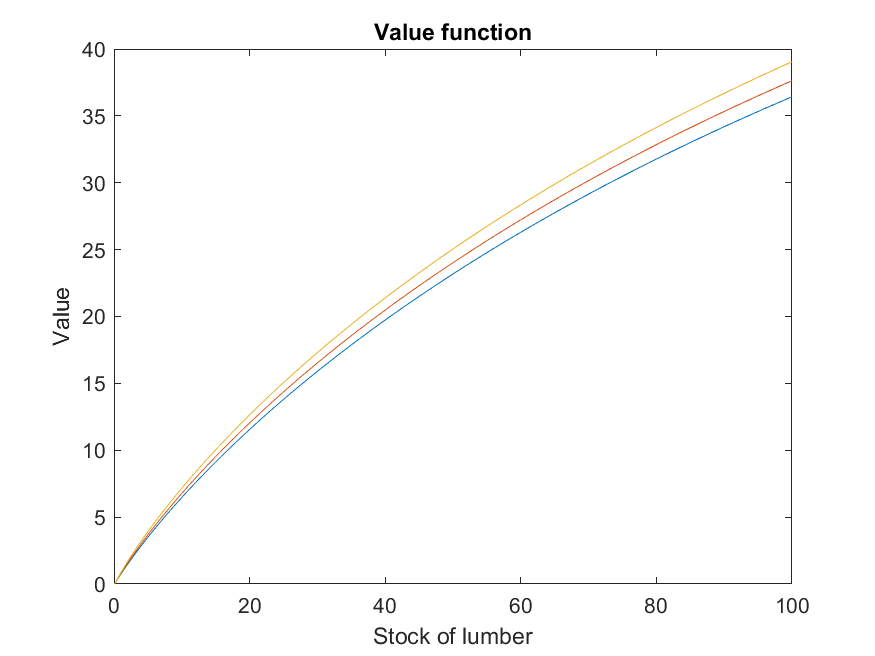
\includegraphics[width=\textwidth]{vf.png}
\caption{The values as a function of lumber stocks, for $p=0.9, 1, 1.1$}
\end{figure}
\clearpage
\section*{Question 4}

\begin{figure}[h]
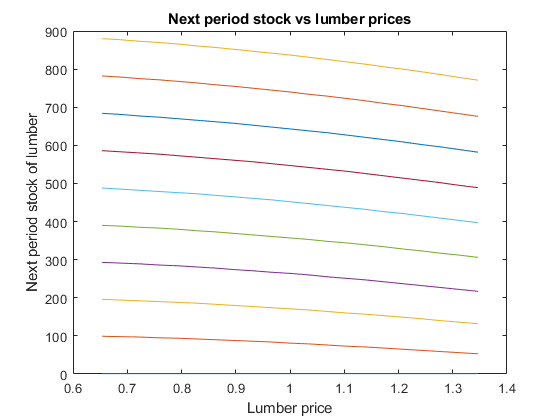
\includegraphics[width=\textwidth]{nextstock.png}
\caption{Next period optimal stocks as a function of lumber prices, for current period stock 0.1, 10.1, 20.1, ..., 90.1}
\end{figure}

\clearpage
\section*{Question 5}
\begin{figure}[h]
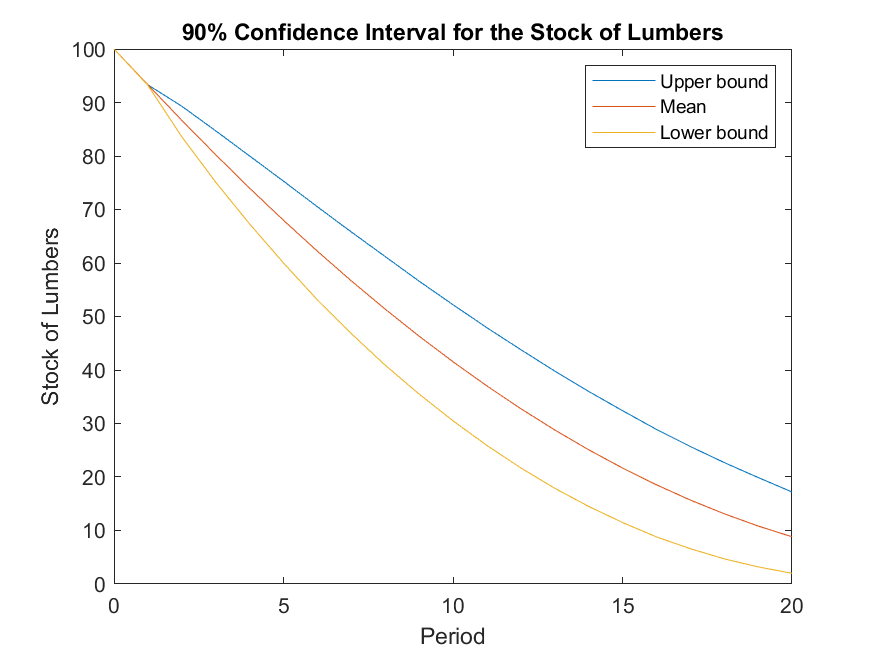
\includegraphics[width=\textwidth]{ci.png}
\caption{Expected stock and 90\% confidence interval}
\end{figure}
\clearpage
\section*{Question 6}
Since $p=0.9, 1.1$ are not on the grid, I draw two curves associated with the closest prices to them in Fig. 4.
\begin{figure}[h]
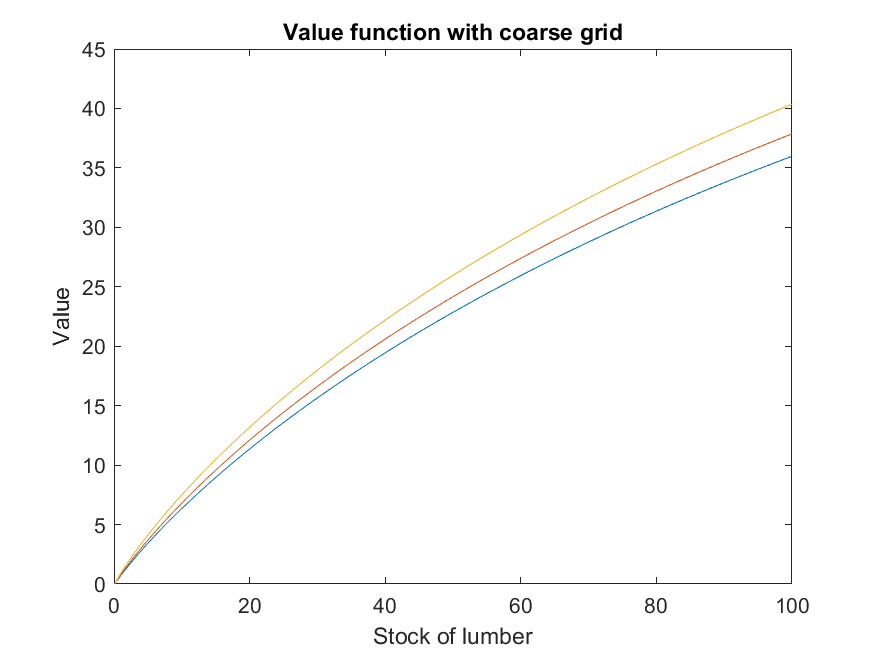
\includegraphics[width=\textwidth]{vf2.png}
\caption{The values as a function of lumber stocks, for $p=0.827, 1, 1.173$}
\end{figure}
\clearpage
\begin{figure}
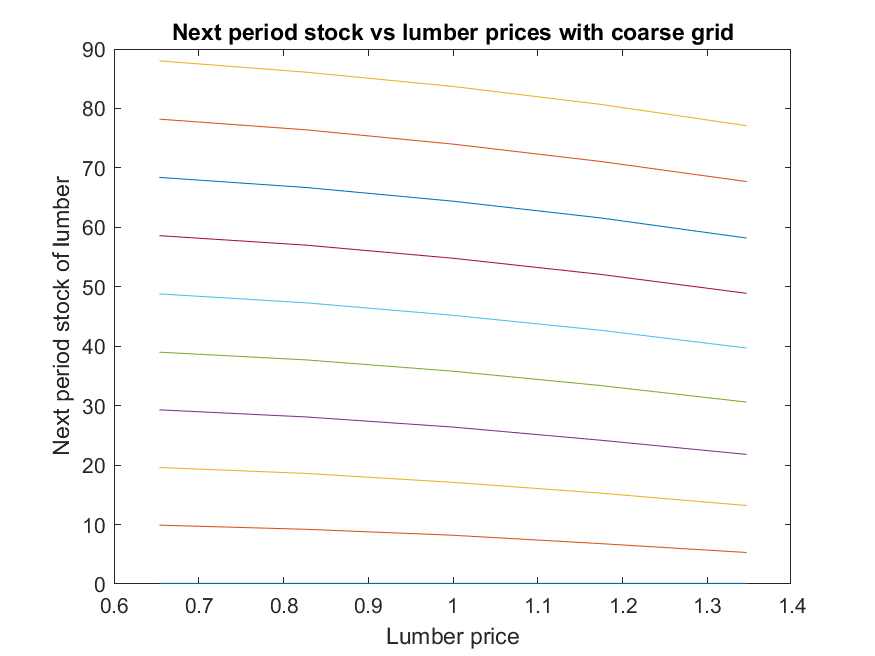
\includegraphics[width=\textwidth]{nextstock2.png}
\caption{Next period optimal stocks as a function of lumber prices, for current period stock 0.1, 10.1, 20.1, ..., 90.1}
\end{figure}
\clearpage
\begin{figure}[h]
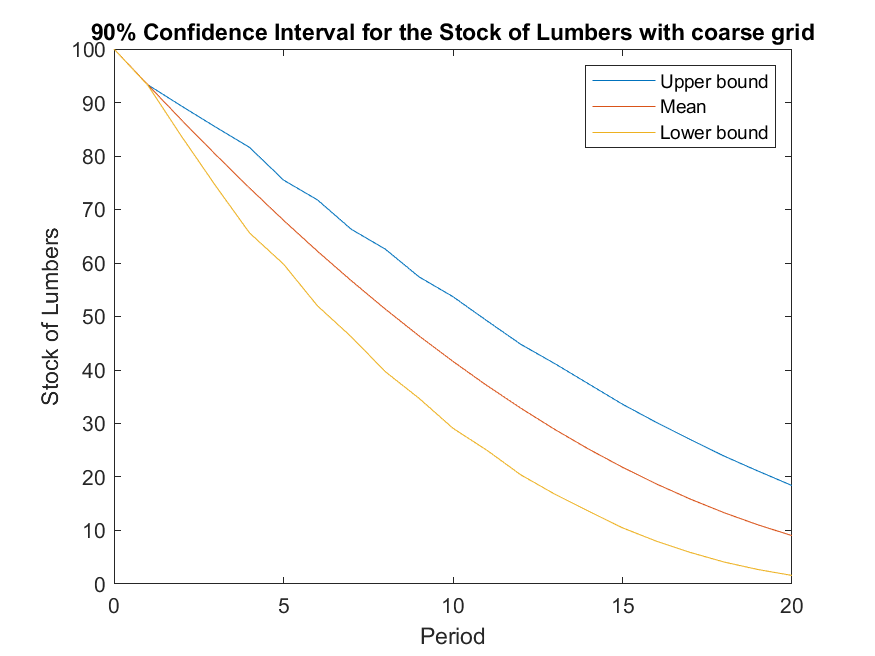
\includegraphics[width=\textwidth]{ci2.png}
\caption{Expected stock and 90\% confidence interval}
\end{figure}
\clearpage
\section*{Code}
\begin{verbatim}
% Motoaki Takahashi
% HW6 Econ 512

clear all
delta = 0.95;
p0 = 0.5;
rho = 0.5;
N = 1000;
k0 = 100; % initial stock of lumber
k = (k0/N):k0/N:k0;

sigmau = 0.1;

%% Question 2
Z = 21; % number of grid points, this must be odd
% Z = 5 % for coarse grid

 
 [prob,grid]=tauchen(Z,p0,rho,sigmau);
disp(['The dimensions of prob are ' num2str(size(prob)) ])
disp(['The dimensions of grid are ' num2str(size(grid)) ])

%% Question 3


v = zeros(N, Z); % initial guess for value function
decision = zeros(N,Z); % this will contain the firm's policy
newv = zeros(N,Z); % this will contain 

%% value function iteration

dif = 1;
tol = 1E-4;
while dif > tol
    EV = v * prob';
    for i = 1:N
        prof = kron(grid, k(i)*ones(N, 1)-k');
        prof(prof < 0) = -1E5; % punish a negative stock of lumber
        inv = k(i)*ones(N, 1)-k';
        inv(inv<0) = 0; % avoid generating an imaginary number
        inv = kron(ones(1, Z), inv);
        prof = prof - 0.2 * inv .^ (1.5); % subtract inv costs from the gross profits
        [vnew(i,:),decision(i,:)]=max(prof + delta * EV);

    end
   dif=norm(vnew-v)/norm(vnew);
   disp(dif)
   v=vnew;
end

%% 
plot(k, v(:, 8), k, v(:, 11), k, v(:, 14)) % for grid Z = 21
% plot(k, v(:, 2), k, v(:, 3), k, v(:, 4)) % for coarse grid Z = 5
title('Value function')
xlabel('Stock of lumber')
ylabel('Value')
saveas(gcf,'vf.png')

%% Question 4

% compute decision rule

drule=zeros(N,Z);

for i=1:Z
    drule(:,i)=k(decision(:,i))';
end

plot(grid, drule(1,:), grid, drule(101,:), grid, drule(201,:), grid, drule(301,:), grid, drule(401,:), grid, drule(501,:), grid, drule(601,:),grid, drule(701,:),grid, drule(801,:), grid, drule(901,:))

title('Next period stock vs lumber prices')
xlabel('Lumber price')
ylabel('Next period stock of lumber')
saveas(gcf,'nextstock.png')

%% Question 5

% Construct the transition matrix from (p, k) pairs to (p', k') pairs
% taken from stochgrow.m
P=zeros(Z*N,Z*N);
T = 21; % the number of periods, including the initial

for i=1:Z
    for j=1:Z
        P((i-1)*N+1:i*N,(j-1)*N+1:j*N)=prob(i,j)*(kron(ones(1,N),drule(:,i))==kron(ones(N,1),k));
    end
end

% the initial state is (p, k)=(1, 100)
state = zeros(1, N*Z);
state(1, ((Z+1)/2)*N) = 1; % this is valid as long as Z is odd

% generate the distribution of p and k for T-1 remaining periods
% and keep track of the CI for k

ci = zeros(3, T); % this will contain the mean and 90% CI for k
ci(:,1) = 100 *ones(3,1);

for t=2:T
    next_state = state * P; %the next period's distribution of states
    dist_kp = zeros(N, Z); % this will contain the joint distribution of k and p in period t
    for i = 1:Z
        dist_kp(:, i) = next_state((i-1)*N+1:i*N)';
    end
    dist_k = sum(dist_kp'); % the marginal dist of k, which is the sum of dist_kp in the p dimension
    clear dist_kp
    mean = dist_k * k'; % mean of k's in period t
    dist_k = cumsum(dist_k); % get the cumulative dist of k
    
    lo = max(find(dist_k<=0.05)); % the index for the 5-percentile
    hi = min(find(dist_k>=0.95)); % the index for 95-percentile
    
    lo = k(lo); % 5-percentile
    hi = k(hi); % 95-percentile
    ci(:,t) = [hi; mean; lo];
    clear hi mean lo
    state = next_state;
end

plot(0:T-1, ci(1,:), 0:T-1, ci(2,:), 0:T-1, ci(3,:))
title('90% Confidence Interval for the Stock of Lumbers')
xlabel('Period')
ylabel('Stock of Lumbers')
legend( 'Upper bound', 'Mean', 'Lower bound')
saveas(gcf,'ci.png')



%% Question 6

% for question 6, redo with Z = 5
\end{verbatim}
\clearpage
\section*{Diary}
\begin{verbatim}
The dimensions of prob are 21  21
The dimensions of grid are 1  21
     1

    0.4373

    0.2763

    0.1986

    0.1507

    0.1173

    0.0920

    0.0720

    0.0557

    0.0428

    0.0327

    0.0249

    0.0191

    0.0146

    0.0112

    0.0086

    0.0065

    0.0049

    0.0037

    0.0028

    0.0020

    0.0015

    0.0011

   7.5347e-04

   5.2416e-04

   3.5831e-04

   2.4048e-04

   1.5836e-04

   1.0230e-04

   6.4817e-05
\end{verbatim}
\end{document}